
For the purpose of this thesis, the Python script was developed to calculate quench velocity assuming that it constant or it is calculated numerically (case a and c). The creation of a numerical map for the quench velocity will be further described in chapter \ref{section:skew_quadrupole_quench_detection_analysis}. This method is used for quench velocity modelling of a skew quadrupole.

This part describes the implementation of quench velocity modelling in ANSYS by means of external Python scripts. Python architecture is designed to perform the following tasks: 

\begin{itemize}
\item launch ANSYS simulation,
\item create APDL scripting commands in order to communicate with ANSYS,
\item create 3D ANSYS meshed geometry of a magnet with given geometrical specifications,
\item map meshed 3D ANSYS geometry to create 1D imaginary coil in Python with specified position of each node,
\item assign material properties to ANSYS geometry with respect to an external magnetic field map,
\item calculate quench velocity at each time step, 
\item assign quenched zone to newly quenched nodes,
\item detect quench at new windings due to turn-to-turn propagation in the 3D ANSYS geometry.
\end{itemize}
 
The simulation is carried out in ANSYS in "-aas" mode (batch mode) while Python main execution script controls it. Except for the above-mentioned tasks, Python script is also in charge of the majority of post-processing. ANSYS sends the results as well as the data about mesh by means of text files which are uploaded to Python as $numpy$ arrays afterwards. The exemplary ANSYS compilation with Python is presented in Appendix \ref{appendix:python_ansys_compilation}. The Python script architecture is depicted in Fig. \ref{fig:python_script_architecture}.

\begin{figure}[H]
\centering
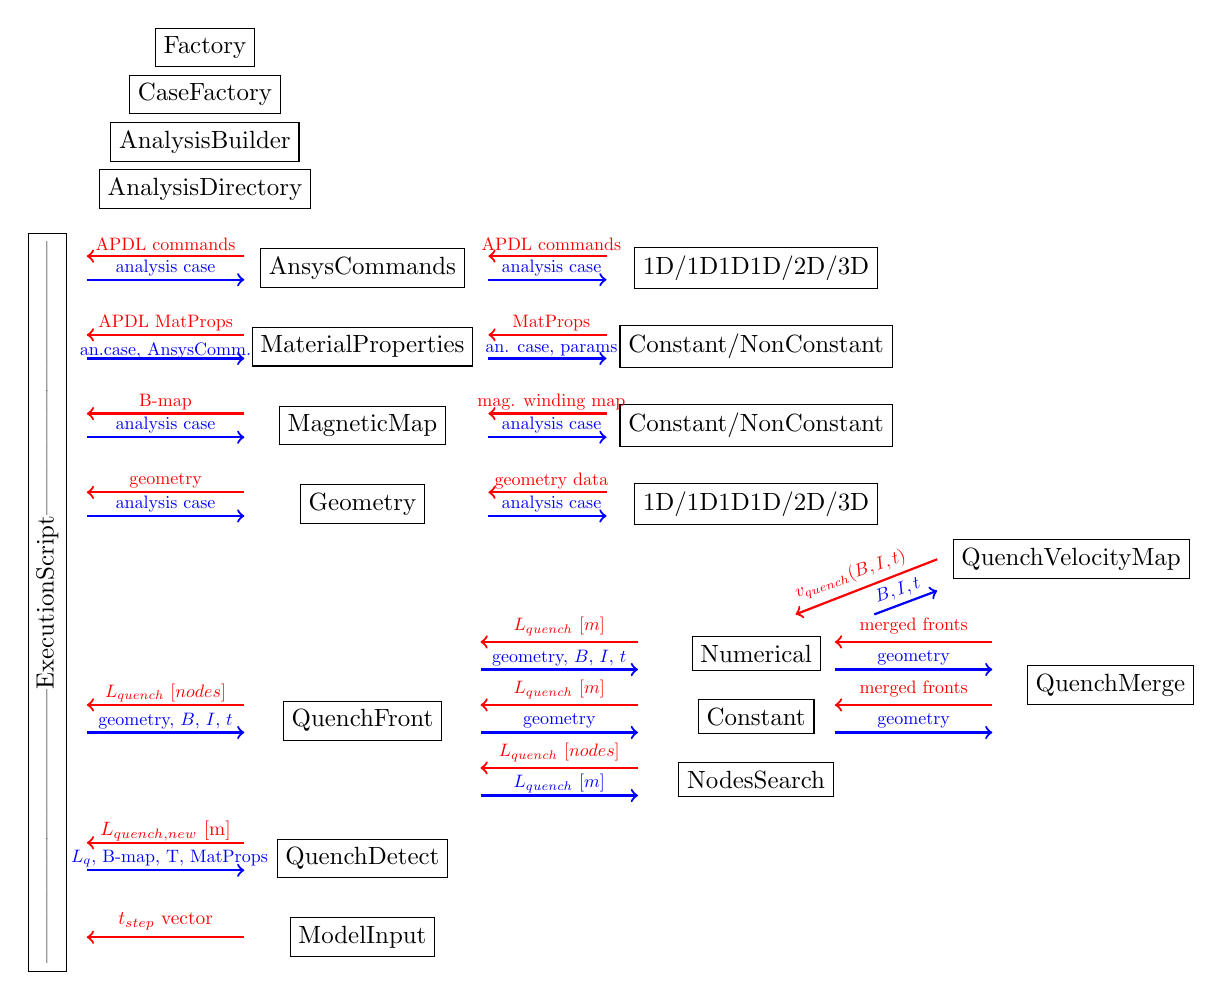
\begin{tikzpicture}[scale = 1]
\node[scale = 0.9, rotate=90] at (1,-4.25) [draw] {|||||||||||ExecutionScript|||||||||||};

\node[scale = 0.9] at (3,2.8) [draw] {Factory};
\node[scale = 0.9] at (3,2.2) [draw] {CaseFactory};
\node[scale = 0.9] at (3,1.6) [draw] {AnalysisBuilder};
\node[scale = 0.9] at (3,1) [draw] {AnalysisDirectory};

\node[scale = 0.9] at (5,0) [draw] {AnsysCommands};
\node[scale = 0.9] at (10,0) [draw] {1D/1D1D1D/2D/3D};
\draw [thick, red, ->] (3.5,0.15) -- (1.5,0.15);
\node[scale = 0.65, red] at (2.5,0.3) {APDL commands};
\draw [thick, blue, ->] (1.5,-0.15) -- (3.5,-0.15);
\node[scale = 0.65, blue] at (2.5,0) {analysis case};
\draw [thick, red, ->] (8.1,0.15) -- (6.6,0.15);
\node[scale = 0.65, red] at (7.4,0.3) {APDL commands};
\draw [thick, blue, ->] (6.6,-0.15) -- (8.1,-0.15);
\node[scale = 0.65, blue] at (7.4,0) {analysis case};

\node[scale = 0.9] at (5,-1) [draw] {MaterialProperties};
\node[scale = 0.9] at (10,-1) [draw] {Constant/NonConstant};
\draw [thick, red, ->] (3.5,-0.85) -- (1.5,-0.85);
\node[scale = 0.65, red] at (2.5,-0.7) {APDL MatProps};
\draw [thick, blue, ->] (1.5,-1.15) -- (3.5,-1.15);
\node[scale = 0.65, blue] at (2.5,-1.05) {an.case, AnsysComm.};
\draw [thick, red, ->] (8.1,-0.85) -- (6.6,-0.85);
\node[scale = 0.65, red] at (7.4,-0.7) {MatProps};
\draw [thick, blue, ->] (6.6,-1.15) -- (8.1,-1.15);
\node[scale = 0.65, blue] at (7.4,-1.05) {an. case, params};

\node[scale = 0.9] at (5,-2) [draw] {MagneticMap};
\node[scale = 0.9] at (10,-2) [draw] {Constant/NonConstant};
\draw [thick, red, ->] (3.5,-1.85) -- (1.5,-1.85);
\node[scale = 0.65, red] at (2.5,-1.7) {B-map};
\draw [thick, blue, ->] (1.5,-2.15) -- (3.5,-2.15);
\node[scale = 0.65, blue] at (2.5,-2) {analysis case};
\draw [thick, red, ->] (8.1,-1.85) -- (6.6,-1.85);
\node[scale = 0.65, red] at (7.4,-1.7) {mag. winding map};
\draw [thick, blue, ->] (6.6,-2.15) -- (8.1,-2.15);
\node[scale = 0.65, blue] at (7.4,-2) {analysis case};

\node[scale = 0.9] at (5,-3) [draw] {Geometry};
\node[scale = 0.9] at (10,-3) [draw] {1D/1D1D1D/2D/3D};
\draw [thick, red, ->] (3.5,-2.85) -- (1.5,-2.85);
\node[scale = 0.65, red] at (2.5,-2.7) {geometry};
\draw [thick, blue, ->] (1.5,-3.15) -- (3.5,-3.15);
\node[scale = 0.65, blue] at (2.5,-3) {analysis case};
\draw [thick, red, ->] (8.1,-2.85) -- (6.6,-2.85);
\node[scale = 0.65, red] at (7.4,-2.7) {geometry data};
\draw [thick, blue, ->] (6.6,-3.15) -- (8.1,-3.15);
\node[scale = 0.65, blue] at (7.4,-3) {analysis case};

\node[scale = 0.9] at (5,-5.75) [draw] {QuenchFront};
\draw [thick, red, ->] (3.5,-5.55) -- (1.5,-5.55);
\node[scale = 0.65, red] at (2.5,-5.4) {$L_\text{quench}~\text{[nodes]}$};
\draw [thick, blue, ->] (1.5,-5.9) -- (3.5,-5.9);
\node[scale = 0.65, blue] at (2.5,-5.75) {geometry, $B$, $I$, $t$};

\node[scale = 0.9] at (10,-4.9) [draw] {Numerical};
\draw [thick, red, ->] (8.5,-4.75) -- (6.5,-4.75);
\draw [thick, blue, ->] (6.5,-5.1) -- (8.5,-5.1);
\node[scale = 0.65, red] at (7.5,-4.55) {$L_\text{quench}~\text{[m]}$};
\node[scale = 0.65, blue] at (7.5,-4.95) {geometry, $B$, $I$, $t$};

\node[scale = 0.9] at (10,-5.7) [draw] {Constant};
\draw [thick, red, ->] (8.5,-5.55) -- (6.5,-5.55);
\draw [thick, blue, ->] (6.5,-5.9) -- (8.5,-5.9);
\node[scale = 0.65, red] at (7.5,-5.35) {$L_\text{quench}~\text{[m]}$};
\node[scale = 0.65, blue] at (7.5,-5.75) {geometry};

\node[scale = 0.9] at (10,-6.5) [draw] {NodesSearch};
\draw [thick, red, ->] (8.5,-6.35) -- (6.5,-6.35);
\draw [thick, blue, ->] (6.5,-6.7) -- (8.5,-6.7);
\node[scale = 0.65, red] at (7.5,-6.15) {$L_\text{quench}~\text{[nodes]}$};
\node[scale = 0.65, blue] at (7.5,-6.55) {$L_\text{quench}~\text{[m]}$};

\node[scale = 0.9] at (14.5,-5.3) [draw] {QuenchMerge};
\draw [thick, red, ->] (13,-4.75) -- (11,-4.75);
\draw [thick, blue, ->] (11,-5.1) -- (13,-5.1);
\node[scale = 0.65, red] at (12,-4.55) {merged fronts};
\node[scale = 0.65, blue] at (12,-4.95) {geometry};

\draw [thick, red, ->] (13,-5.55) -- (11,-5.55);
\draw [thick, blue, ->] (11,-5.9) -- (13,-5.9);
\node[scale = 0.65, red] at (12,-5.35) {merged fronts};
\node[scale = 0.65, blue] at (12,-5.75) {geometry};

\node[scale = 0.9] at (14,-3.7) [draw] {QuenchVelocityMap};
\draw [thick, red, ->] (12.3,-3.7) -- (10.5,-4.4);
\draw [thick, blue, ->] (11.5,-4.4) -- (12.3,-4.1);
\node[scale = 0.65, red, rotate=19] at (11.2,-3.9) {$v_\text{quench} (B,I,t)$};
\node[scale = 0.65, blue, rotate=19] at (11.8,-4.1) {$B,I,t$};

\node[scale = 0.9] at (5,-7.5) [draw] {QuenchDetect};
\draw [thick, red, ->] (3.5,-7.3) -- (1.5,-7.3);
\draw [thick, blue, ->] (1.5,-7.65) -- (3.5,-7.65);

\node[scale = 0.7, red] at (2.5,-7.15) {$L_\text{quench, new}$ [m]};
\node[scale = 0.65, blue] at (2.55,-7.5) {$L_\text{q}$, B-map, T, MatProps};

\node[scale = 0.9] at (5,-8.5) [draw] {ModelInput};
\draw [thick, red, ->] (3.5,-8.5) -- (1.5,-8.5);
\node[scale = 0.7, red] at (2.5,-8.3) {$t_\text{step}$ vector};
\end{tikzpicture}
\caption{Python script architecture}
\label{fig:python_script_architecture}
\end{figure}

Fig. \ref{fig:python_script_architecture} describes the Python code consisting of 4 different Classes and one executive script. The \textit{executive\_script} launches the simulation and executes pre-processing, solution as well as post-processing part of ANSYS simulation. It uses the Class \textit{ansys} to translate Python functions into APDL scripting language. The Class \textit{geometry} imports a meshed geometry and assigns the position in space for each node. Then, the class \textit{quench\_velocity} assigns new quench front position at each time step depending on a current quench velocity. Since the Class \textit{quench\_velocity} operates in meters, it requires a separate class \textit{node\_search} which maps a node number for the calculated quench length as described in Section \ref{subsection:node_searching_algorithm}.\\

At this stage, the class \textit{quench\_velocity} assumes that the quench velocity is constant. In further steps, the quench velocity will be estimated in two-way coupling manner as described in Section \ref{subsection:quench_velocity_algorithm}. In order to reach this step, a new Class called \textit{quench\_detection} will be created. It will initialize the new quench front as soon as the critical temperature is achieved outside of the quenched zone of the coil (turn to turn heat propagation).